\section{Aufbau und Durchführung}
\subsection{Aufbau}
\label{sec:Aufbau}
Zur Untersuchung des Brechungsindex in Abhängigkeit der Wellenlänge wird ein Prismen-Spektralapparat verwendet, wie er in Abbildung \ref{fig:1} dargestellt ist.

\begin{figure}[H]
  \centering
  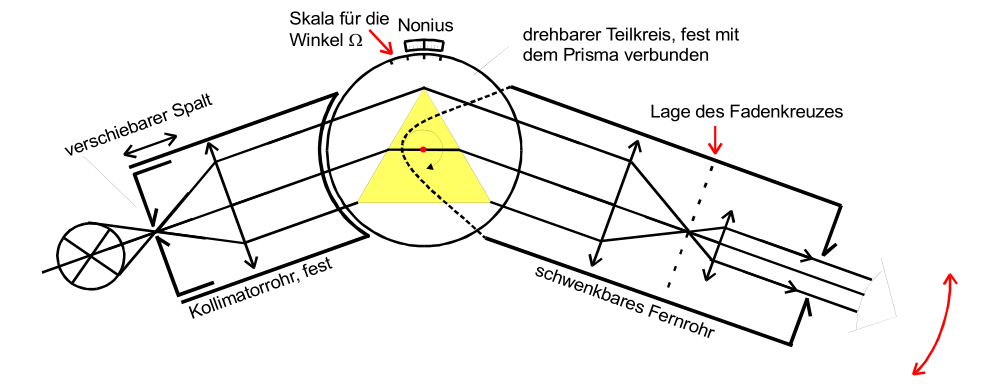
\includegraphics[height=4cm]{ressources/aufbau.png}
  \caption{Darstellung des verwendeten Spektralapparates. \cite{skript}}
  \label{fig:1}
\end{figure}

Prinzipiell besteht dieser aus einem Glasprisma, welches sich im Zentrum eines zweiarmigen Goniometers befindet.
Am Anfang des linken Armes, der im Versuch fest steht, befindet sich eine Quecksilber-Cadmium-Dampflampe.
Das Lichtbündel passiert ein Spalt-/Linsensystem, sodass ein aufgeweiteter Strahl entsteht.
Dieser wandert weiter auf das drehbare Mittelstück, auf dem sich das Prisma befindet.
Es ist mit einer Winkelskala zusätzlich Nonius versehen.
Das gebrochene Licht kann daraufhin mit dem zweiten schwenkbaren Arm aufgefangen werden.
Durch ein Linsensystem mit eingebautem Fadenkreuz können somit die Spektrallinien angepeilt werden.
